%************************************************
\chapter{Passive and Active Communications}\label{ch:passive_com}
%************************************************

In a previous chapter we learned how to exchange data with the server, since \ac{XML} and \ac{JSON} can be used for receiving as well as transmitting information.

There are two ways in which a cloud service can communicate with an application, the application can actively query the server for new information every couple of minutes or the server can passively send information to the application, without the need for interaction.

This premise builds upon the ideas discussed in the previous chapter, since it makes use of asynchronous, bidirectional communications as well as normal HTTP requests.

\section{Active Communications}
Active Communications are very straight-forward. When the user interacts with the application and it needs to collect more data, the application makes an active request to the server asking it for this information. Examples for this behavior are searches or when the user wants to update a view with the latest information from the server. In an application like Twitter, this can be when the user refreshes the activity feed or when he searches for something.

The application can also actively send data and, if the server allows it, manipulate the data on the server. Keeping with the Twitter example, a user can create a new tweet, follow users, manipulate existing tweets and interact with other users. All of these are examples of active communications in action.

\section{Passive Communications}
On the other hand, Passive Communications require no interaction on the user part whatsoever. The server handles all the communication and administers how, when and to whom the notifications are sent.

In mobile environments, Passive Communications are often referred to as \textit{Push Notifications}, because they are "pushed" to the device rather than actively "pulled".

There are many ways of generating push notifications:
\begin{itemize}
\item You can implement your own receiver inside the application using Websockets and have a server send the notifications over this channel.
\item You can use any of the many third party libraries that handle the implementation and offer some kind of web service to handle notifications.
\item Use Google's and Apple's own services that let you easily send notifications to your users.
\end{itemize}

Each of these methods has its pros and cons, but if you want a great amount of flexibility, without the hassle of creating everything yourself, you should use Google's and Apple's own implementation. The only downside of this approach is that we can't share this code and have to implement everything twice.


\section{Our Use Case}

The use of active communications within our application is pretty obvious. The application connects to the server periodically to get new job vacancies and new companies, if there are any, and when the user searches for something specific.

The special use case comes with the push notifications. We want the user to receive a notification when a new vacancy matching the user's previous searches is posted.

In order to send the notifications, we need to add the specific implementation of each service to the application.

\begin{figure}[bth]
        \myfloatalign
        \subfloat[Google Cloud Messanging]
        {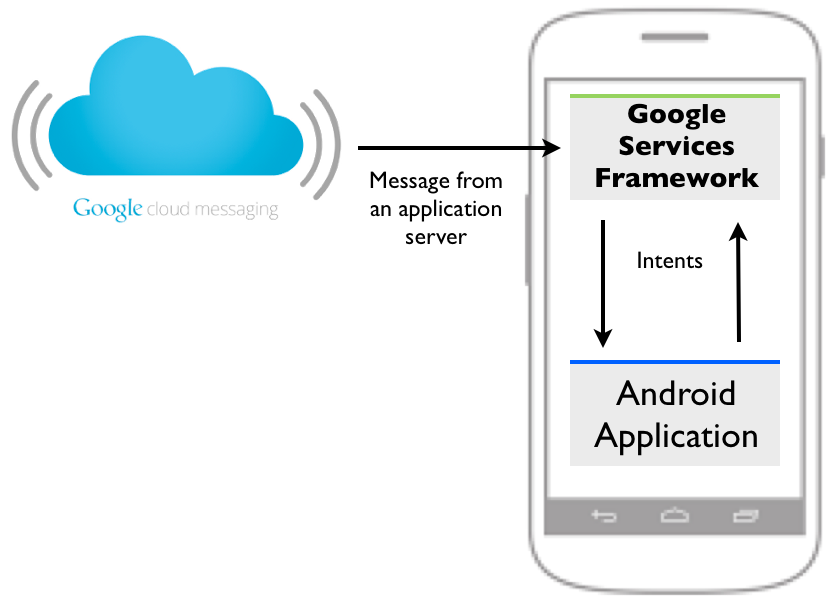
\includegraphics[width=.65\linewidth]{gfx/gcm}} \quad
        \subfloat[Apple Push Notification Service]
        {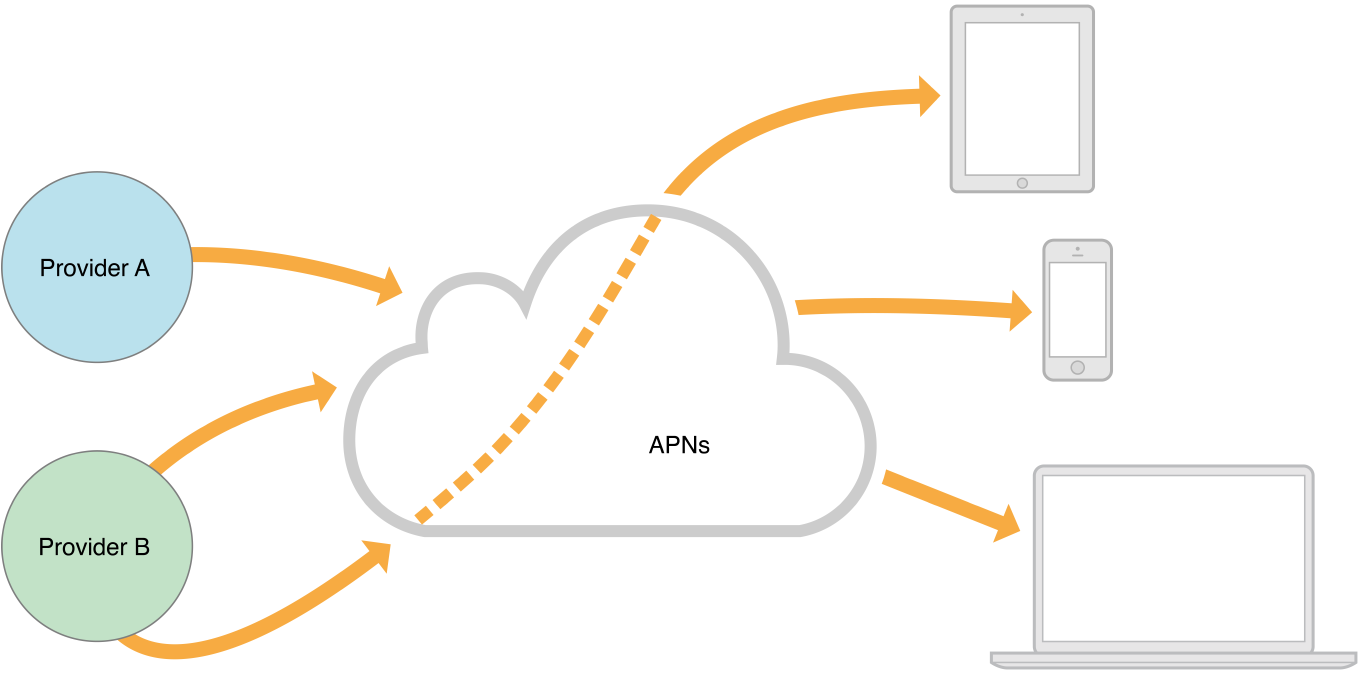
\includegraphics[width=.65\linewidth]{gfx/apns}} \\
        \caption[Cloud Messaging Services]{Cloud Messaging Services}\label{fig:push}
\end{figure}  






